\documentclass{ctexart}
\usepackage{geometry}
\usepackage{fancyhdr}
\usepackage{graphicx}
\usepackage{booktabs}
\usepackage{amsmath}
\usepackage{tikz}
\usepackage{array}
\xeCJKsetup{CJKmath=true} 
\usepackage{zhnumber} % change section number to chinese
\renewcommand\thesection{\zhnum{section}}
\renewcommand \thesubsection {\arabic{subsection}}
\CTEXsetup[format={\Large\bfseries}]{section}

\geometry{
    a4paper,
    left=3.18cm,
    right=3.18cm,
    top=3.04cm,
    bottom=3.04cm
}

\pagestyle{fancy}
\fancyhf{}
\renewcommand{\headrulewidth}{0.7pt} % 设置页眉横线粗细
\fancyhead[L]{\kaishu\large 大学物理实验报告} % 在左侧设置页眉文字
\fancyhead[R]{\kaishu\large 哈尔滨工业大学(深圳) } % 在右侧设置页眉文字
\fancyfoot[R]{\thepage} % 将页数放在右下角


\setlength\headwidth{\textwidth}

\begin{document}

\noindent
\begin{center}
\textbf{
\begin{tabular}{p{2.4cm}p{2.4cm}p{4cm}p{4cm}}
    班级 \hrulefill & 学号 \hrulefill & 姓名 \hrulefill & 教师签字 \hrulefill \\
\end{tabular}
\begin{tabular}{p{6cm}p{3.6cm}p{3.6cm}}
    实验日期 \hrulefill & 预习成绩 \hrulefill & 总成绩 \hrulefill
\end{tabular}
{\noindent}	 \rule[-10pt]{\textwidth}{0.7pt}
}\end{center}

\begin{center}
    \Large \textbf{实验名称 \underline{霍尔效应及其应用}}
\end{center}

\section{实验目的}
\vspace{4\baselineskip}

\section{实验预习}
\subsection{如何利用霍尔效应测量磁场？}
\vspace{4\baselineskip}
\subsection{霍尔电压测量中存在哪些系统误差？用什么方法消除这些误差？}
\vspace{12\baselineskip}
\subsection{各向异性磁阻：}
\vspace{4\baselineskip}
\newpage

\section{实验现象及数据记录}
\subsection{测量$V_H-I_M$关系}
表格略
\vspace{18\baselineskip}
\subsection{测量$V_H-I_S$关系}
表格略
\newpage

\subsection{测量$V_H-X$关系}
表格略
\newpage

\subsection{$AMR$的$V_OUT-I_M$关系}
表格略
\vspace{12\baselineskip}
\subsection{$AMR$的$V_OUT-\theta$关系}

\begin{tikzpicture}[remember picture,overlay]
    \node[anchor=south east,inner sep=100pt] at (current page.south east) {
        \renewcommand{\arraystretch}{1.5} % 表格行高倍数
        \setlength{\tabcolsep}{18pt}    
    \begin{tabular}{|c|c|}
        \hline
        \LARGE  教师 & \LARGE  姓名 \\
        \hline
        \LARGE \kaishu 签字 &  \\
        \hline
        \end{tabular}
    };
\end{tikzpicture}

\newpage

\section{数据处理及作图}

\subsection{画$V_H-I_M$和$V_H-I_S$曲线，用最小二乘法计算斜率$K$，计算霍尔元件灵敏度$K_H$；}

由表1中的数据可以画出$V_H-I_M$曲线，如图1所示：

\begin{center}
    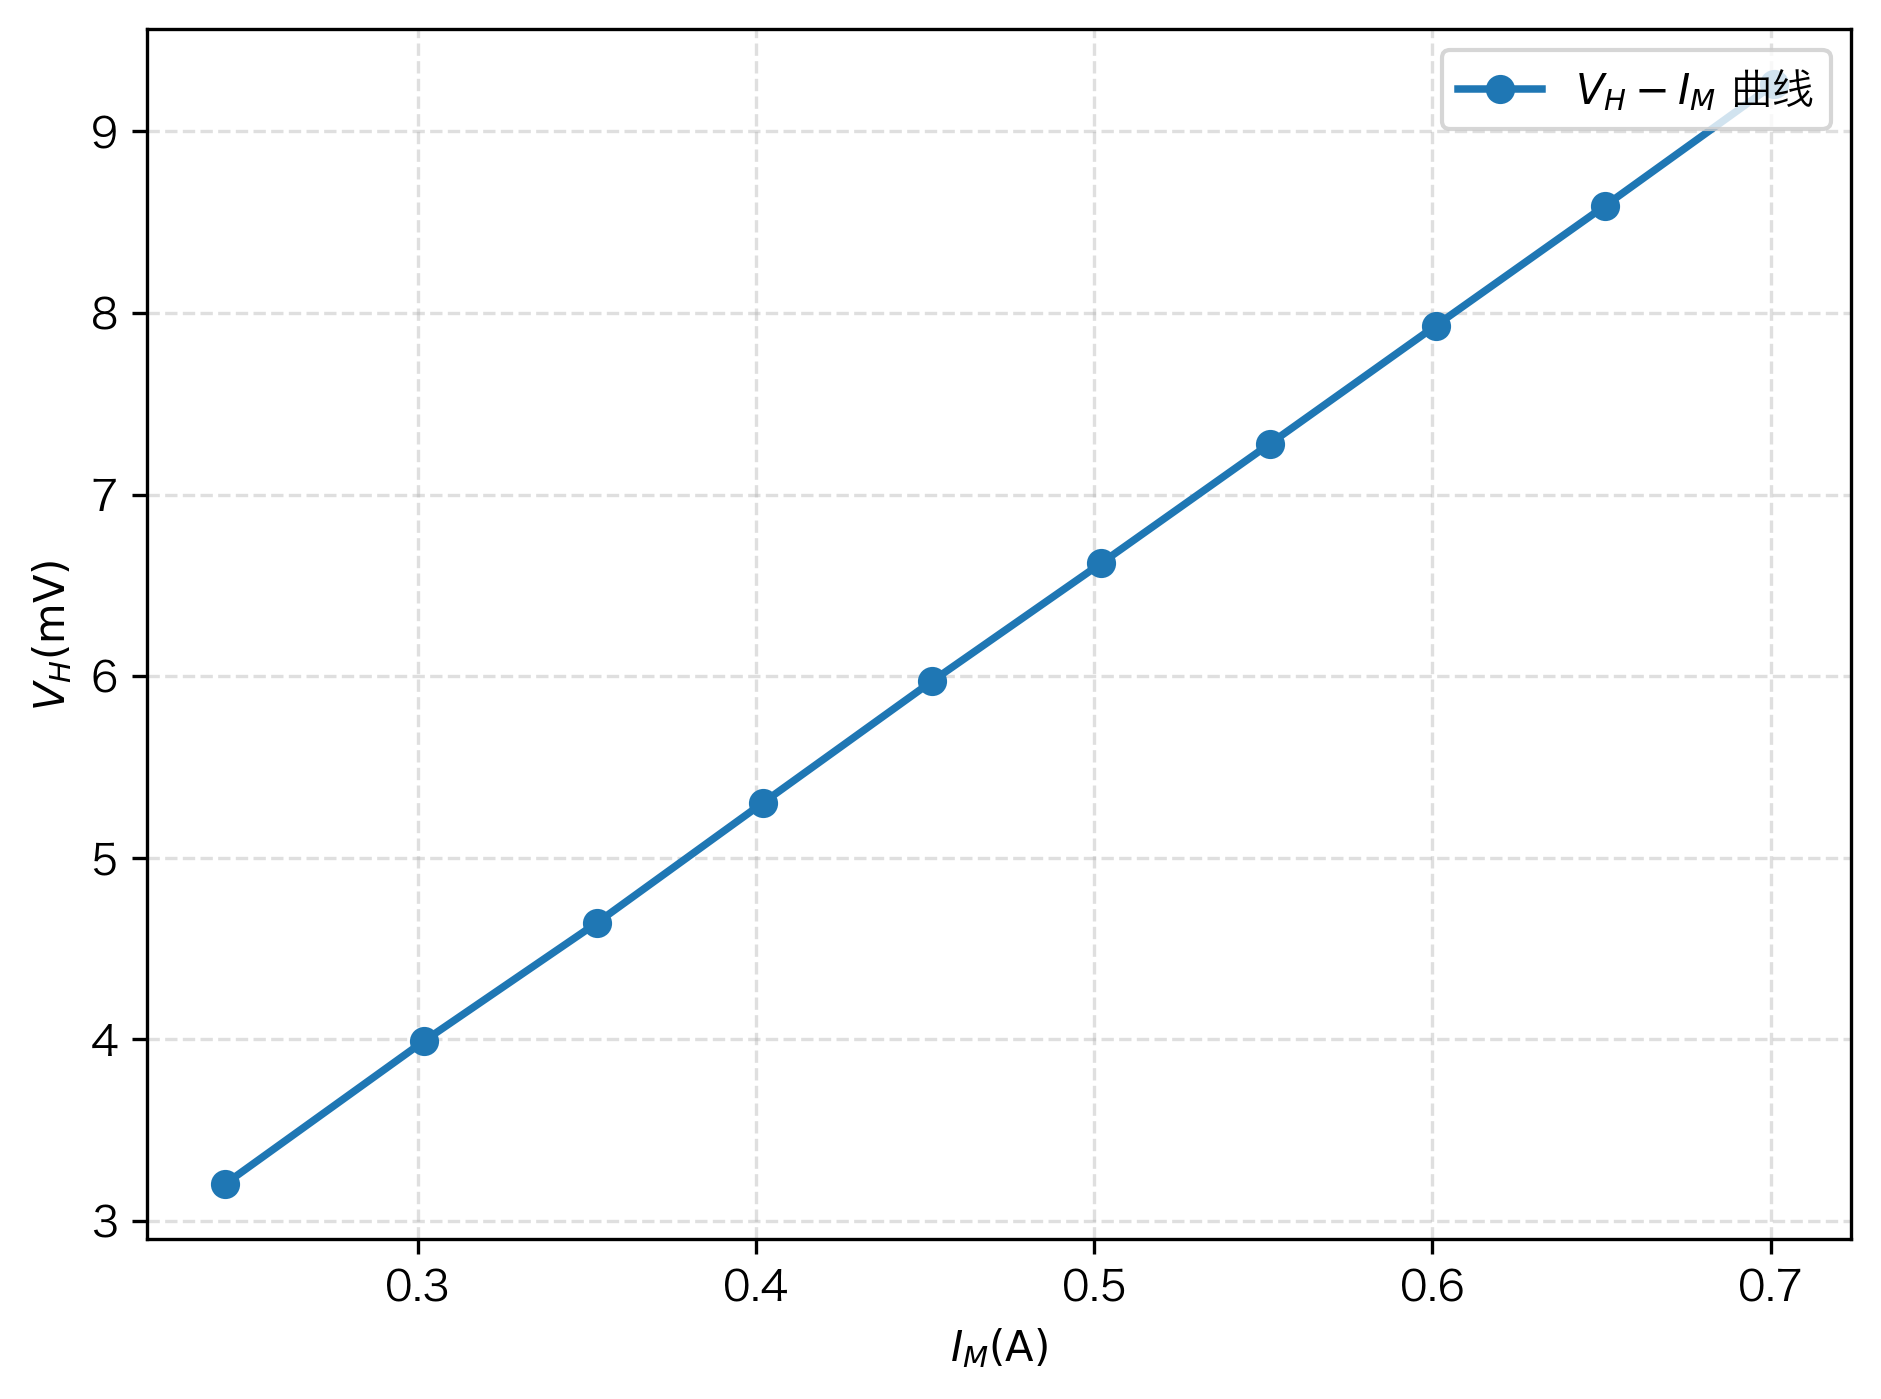
\includegraphics[width=0.78\textwidth]{vh_im_curve.png}
    
    图1 $V_H-I_M$曲线
\end{center}

使用最小二乘法对该组数据进行线性拟合：

\[
\hat{V}_H = \hat{a} + \hat{b} I_M,\qquad
\overline{I}_M = \frac{\sum\limits_{i = 1}^{10} I_{M_i}}{10},\qquad
\overline{V}_H = \frac{\sum\limits_{i = 1}^{10} V_{H_i}}{10}
\]

\[
\hat{b} = \frac{\sum\limits_{i = 1}^{10} I_{M_i} V_{H_i} - 10 \overline{I}_M \overline{V}_H}{\sum\limits_{i = 1}^{10} I_{M_i}^2 - 10 \overline{I}_M^2},\qquad
\hat{a} = \overline{V}_H - \hat{b} \overline{I}_M
\]

可求得

\[
\hat{a} = -0.0126,\qquad
\hat{b} = 13.2184
\]

所以

$$ \hat{V}_H = -0.0126 + 13.2184 I_M $$
$$ K = \hat{b} = 13.2184 $$

由表2中的数据可以画出$V_H-I_S$曲线，如图2所示：

\begin{center}
    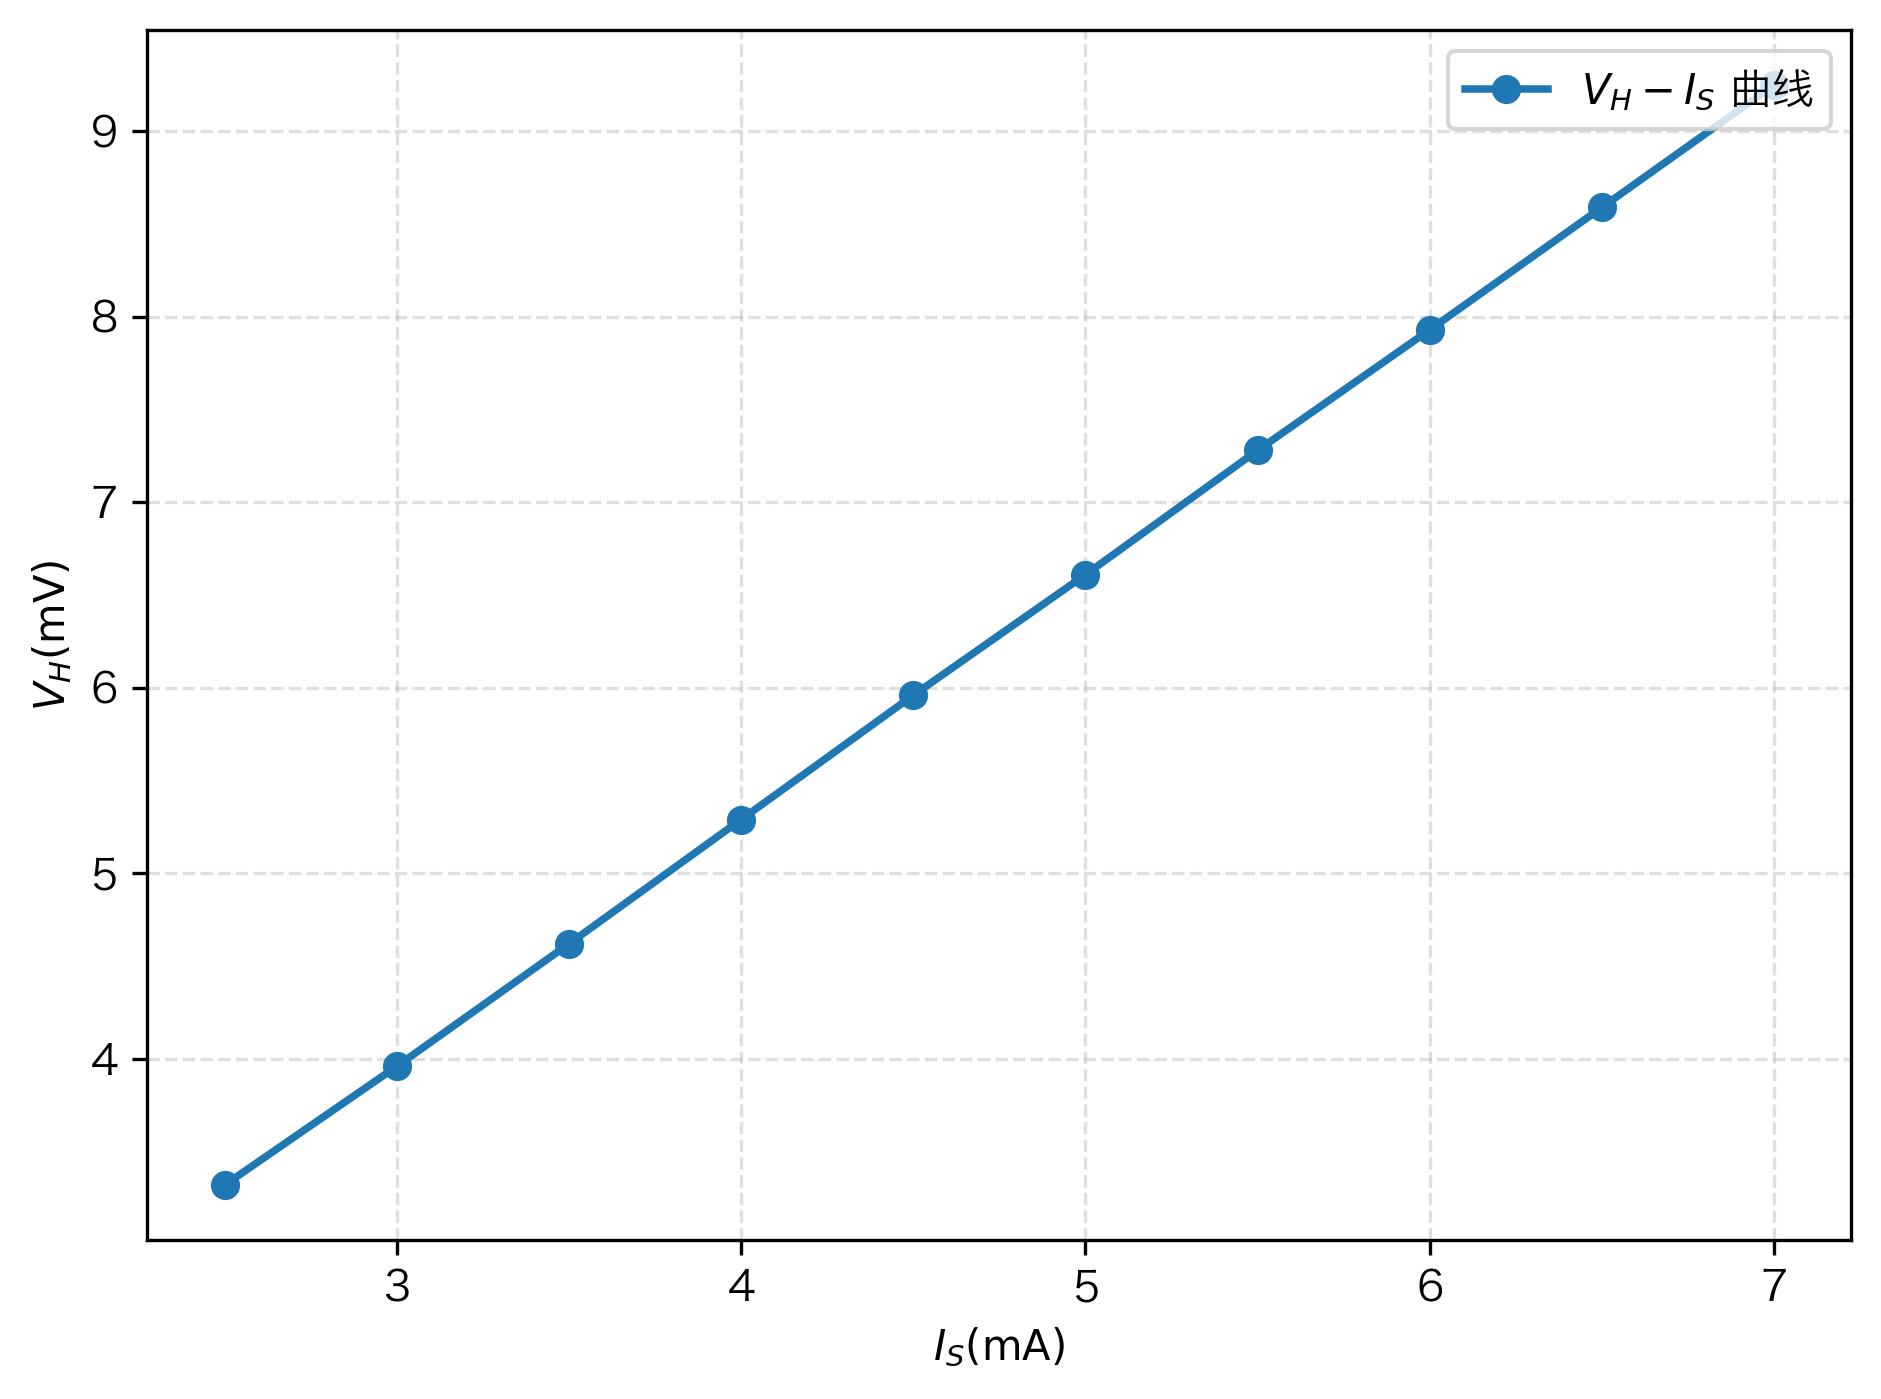
\includegraphics[width=0.78\textwidth]{vh_is_curve.png}
    
    图2 $V_H-I_S$曲线
\end{center}

使用最小二乘法对该组数据进行线性拟合：

\[
\hat{V}_H = \hat{a} + \hat{b} I_S,\qquad
\overline{I}_S = \frac{\sum\limits_{i = 1}^{10} I_{S_i}}{10},\qquad
\overline{V}_H = \frac{\sum\limits_{i = 1}^{10} V_{H_i}}{10}
\]

\[
\hat{b} = \frac{\sum\limits_{i = 1}^{10} I_{S_i} V_{H_i} - 10 \overline{I}_S \overline{V}_H}{\sum\limits_{i = 1}^{10} I_{S_i}^2 - 10 \overline{I}_S^2},\qquad
\hat{a} = \overline{V}_H - \hat{b} \overline{I}_S
\]

可求得

\[
\hat{a} = 0.0081,\qquad
\hat{b} = 1.3206
\]

所以

$$ \hat{V}_H = 0.0081 + 1.3206 I_S $$
$$ K = \hat{b} = 1.3206 $$

由 $V_H = K_H I_S B$ 计算霍尔元件的灵敏度$K_H$：

利用 $V_H-I_M$ 数据，求得：
$$ K_H = \frac{\sum\limits_{i = 1}^{10} \frac{V_{H_i}}{I_S B_i}}{10} = 178.195 \ \mathrm{m^2/C} $$

利用 $V_H-I_S$ 数据，求得：
$$ K_H = \frac{\hat{b}}{B} = 178.431 \ \mathrm{m^2/C} $$

取均值为霍尔元件灵敏度测量值，即

$$ \overline{K_H}= \frac{1}{2}\left(178.195 + 178.431\right) = 178.313 \ \mathrm{m^2/C} $$

\subsection{画$B-X$图，描述螺线圈内$X$方向上$B$的分布特征；}

由表3中的数据可以画出$B-X$曲线，如图3所示：

\begin{center}
    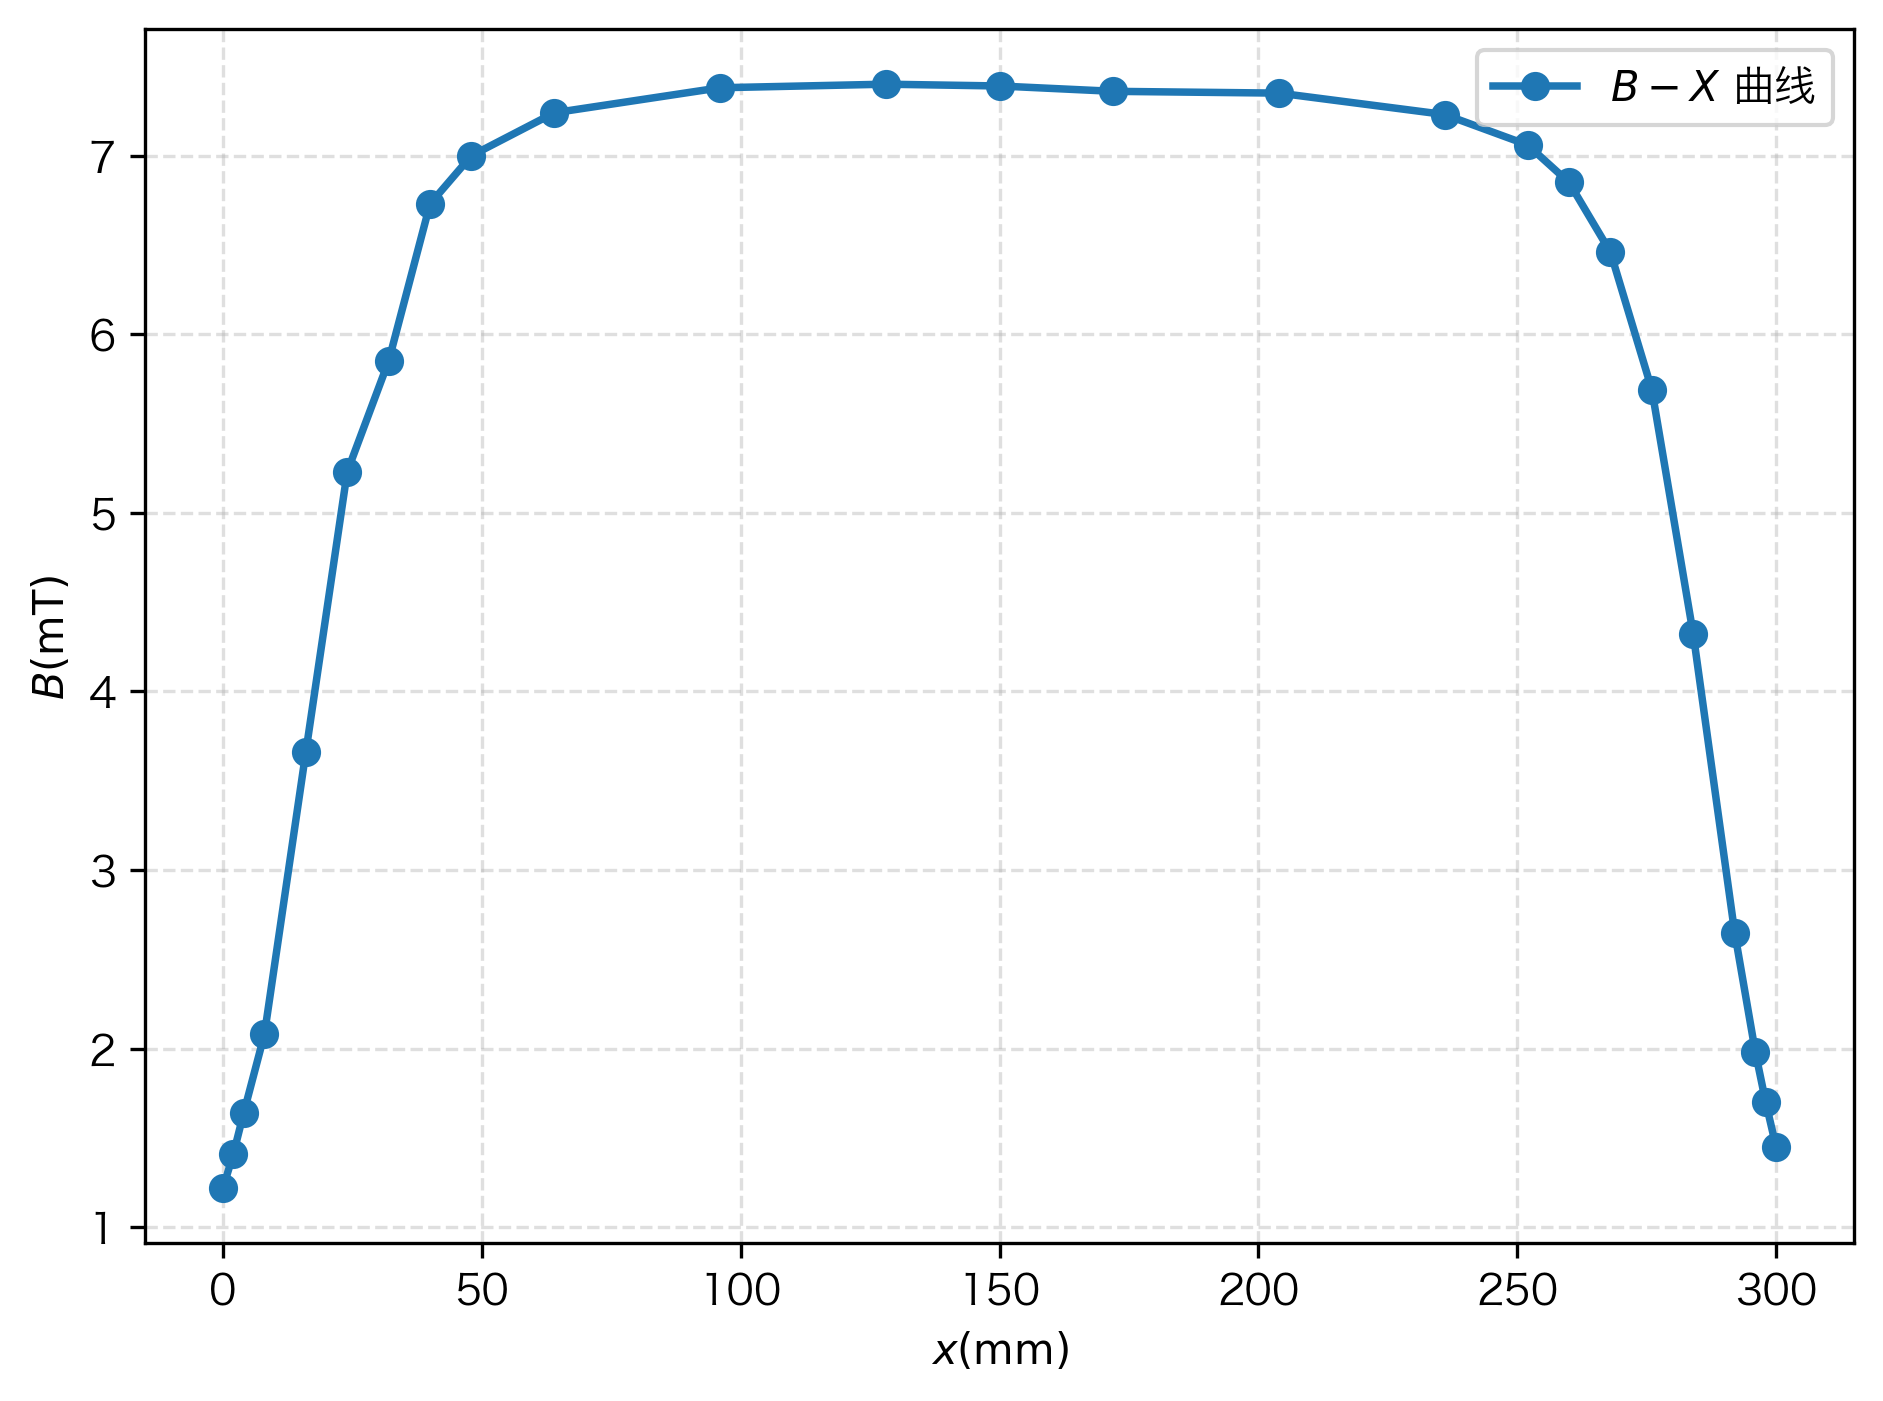
\includegraphics[width=0.78\textwidth]{b_x_curve.png}
    
    图3 $B-X$曲线
\end{center}

由图3可见，磁感应强度$B$随$x$的增大先迅速增大，在螺线圈中部附近达到最大值后变化较缓，形成较平坦的区域；继续向线圈另一端移动时，$B$又迅速减小。说明螺线圈内部中部磁场分布较均匀，而在线圈两端磁场明显减弱，存在边缘效应。

\subsection{作出$V_{OUT}-B$关系曲线，并取在线性范围$\left( \pm 6Gs \right)$内数据，根据公式计算各向异性磁阻传感器的灵敏度$S_A$；}

由表4中的数据可以画出$V_{OUT}-B$曲线，如图4所示：

\begin{center}
    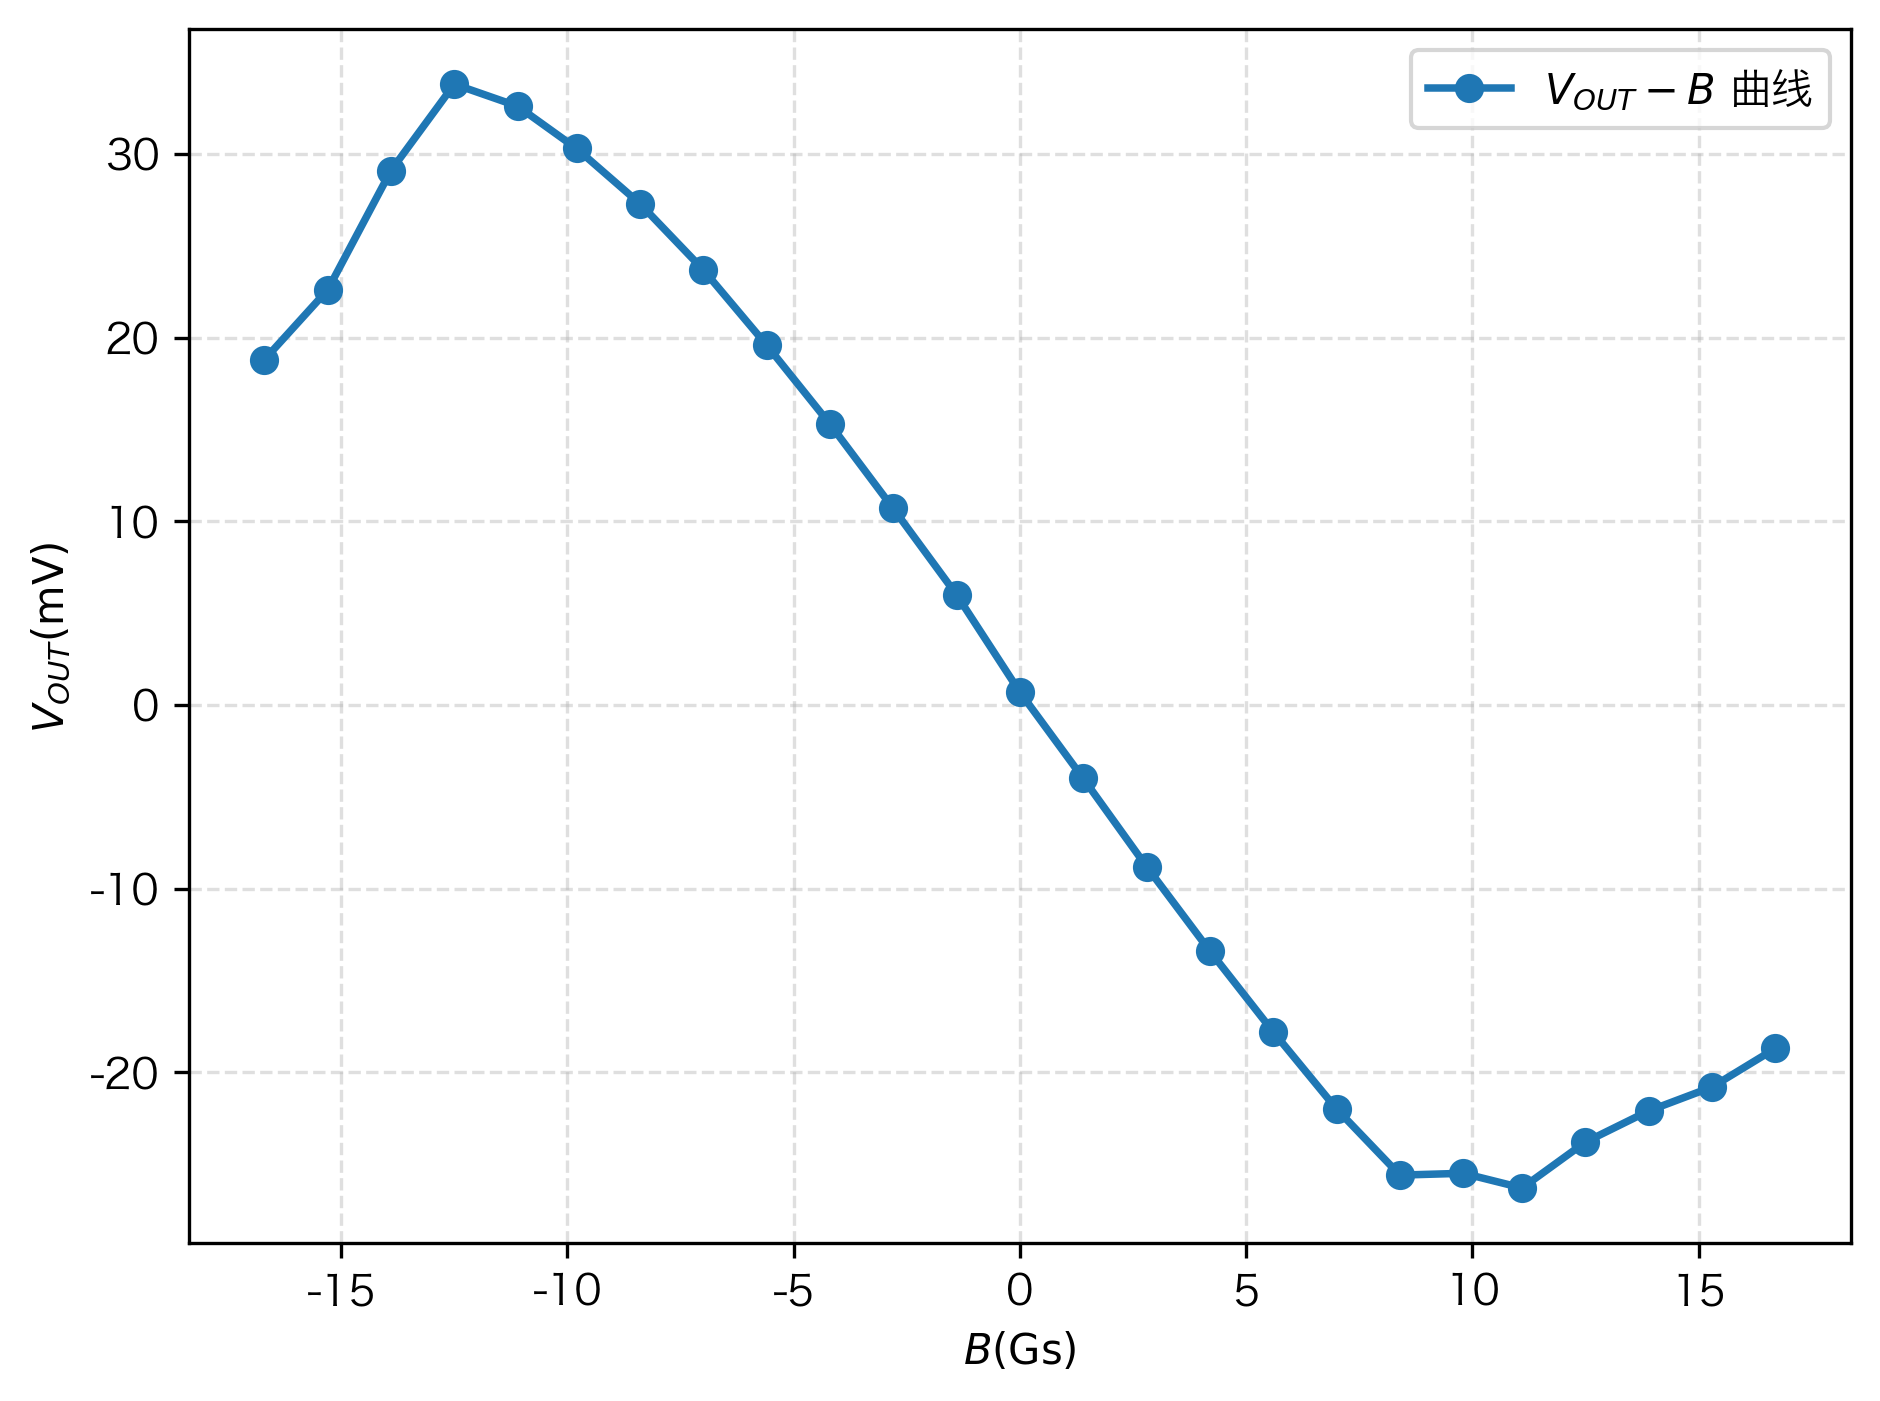
\includegraphics[width=0.78\textwidth]{vout_b_curve.png}
    
    图4 $V_{OUT}-B$曲线
\end{center}

符合线性关系的实验数据组共有 $I_M$ 为 $200mA\sim -200mA$ 的9组数据，对其进行线性拟合，并用最小二乘法计算斜率得 $\mid k \mid = 3.3893$，

再将斜率除以 $V_S$ 即可获得传感器的灵敏度：

$$ S_A = \frac{V_{OUT}}{V_S \cdot B} = 0.847 \ \mathrm{mV/\left(V \cdot Gs\right)} $$

\subsection{作各向异性磁阻传感器的$V_{OUT}-\theta$关系曲线，确认输出电压与转角的关系。}

由表5中的数据可以画出$V_{OUT}-\theta$曲线，如图5所示：

\begin{center}
    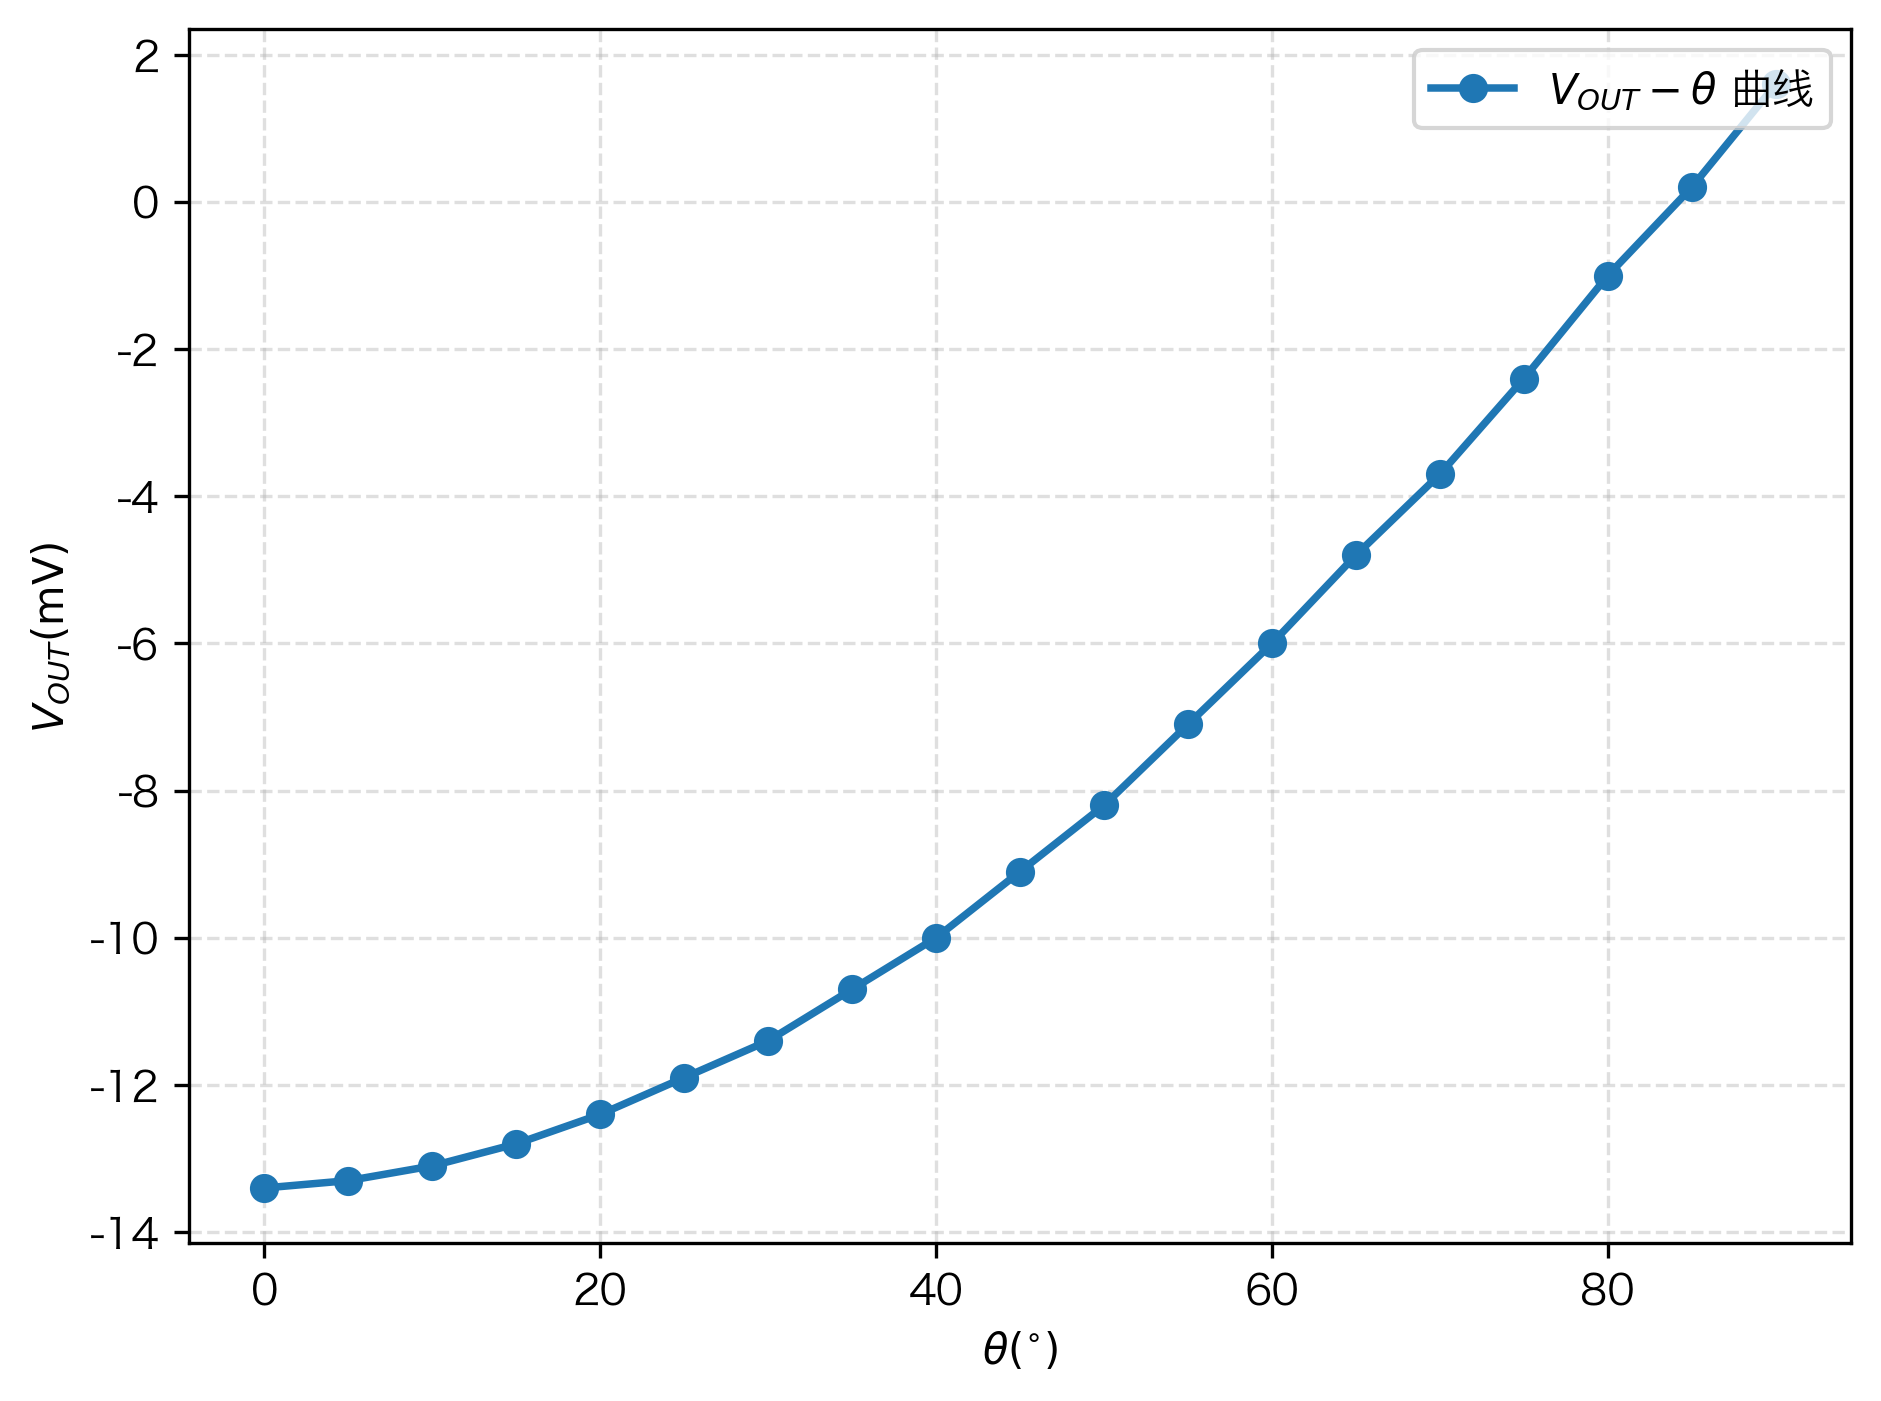
\includegraphics[width=0.78\textwidth]{vout_theta_curve.png}
    
    图5 $V_{OUT}-\theta$曲线
\end{center}


\section{讨论问题}

\subsection{如何根据$B$、$IH$和$UH$方向判断霍尔片的导电类型（N型或P型半导体），要求画图说明。（注：N型半导体中，载流子为电子；P型半导体中将载流子视为正离子）；}

\subsection{估算本实验所用霍尔片的载流子浓度。}

\end{document}
